\documentclass[a4paper,14pt]{extarticle} % the default article class is limited to 12pt, but you can go up to 14, 17 or 20 points if you use the extarticle class:
\usepackage{cmap} % make LaTeX PDF output copy-and-pasteable
\usepackage[T2A]{fontenc}
\usepackage[utf8]{inputenc}
\usepackage[english,ukrainian]{babel}

\usepackage{amssymb,amsfonts,mathtools,amsmath,cite,enumerate,float}
\usepackage{indentfirst} % set an additional space before a paragraph at the begining of new section
\usepackage{setspace}
\usepackage{textcomp}

\setlength{\arrayrulewidth}{0.5mm} % this sets the thickness of the borders of the table
\setlength{\tabcolsep}{18pt} % the space between the text and the left/right border of its containing cell is set to 18pt with this command
\renewcommand{\arraystretch}{1.5} % the height of each row is set to 1.5 relative to its default height

\usepackage{siunitx} % required for alignment
\sisetup{
  round-mode          = places, % rounds numbers
  round-precision     = 4, % to 2 places
}

\usepackage{leftidx}

\usepackage{import} % for adding a file by path https://tex.stackexchange.com/questions/246/when-should-i-use-input-vs-include

\usepackage{geometry} 
\geometry{left=1.25cm}
\geometry{right=1.25cm}
\geometry{top=1cm}
\geometry{bottom=2cm}

\usepackage[table,xcdraw,dvipsnames]{xcolor}
\usepackage{color}
% 1) tutorial about xcolor:  https://www.overleaf.com/learn/latex/Using_colours_in_LaTeX
% 2) huge tutorial about xcolor: https://latex-tutorial.com/color-latex/ 
% 3) RGB calculator: https://www.w3schools.com/colors/colors_rgb.asp

\usepackage{hyperref}
\definecolor{linkcolor}{HTML}{0000FF}
\definecolor{urlcolor}{HTML}{0000FF} 
\hypersetup{pdfstartview=FitH, linkcolor=linkcolor, urlcolor=urlcolor, colorlinks=true}

\usepackage{graphicx}
\usepackage{wrapfig}
\graphicspath{{Images/}} % path to images

\parskip=1mm %space between paragraphs

\usepackage{listingsutf8} % for code (origin: \usepackage{listings})

\lstset{
    frame=single, %lines
    language=Python,
    aboveskip=3mm,
    belowskip=3mm,
    columns=flexible,
    basicstyle={\small\ttfamily},
    numbers=left,
    numberstyle=\tiny\color{gray},
    commentstyle=\color{OliveGreen},
    stringstyle=\color{Mahogany},
    morestring=[b]''',
    showstringspaces=false,
    keywordstyle=\bfseries\color{blue},
    emph={[1]import, as, for, return}, emphstyle={[1]\bfseries\color{magenta}},
    emph={[2]range}, emphstyle={[2]\bfseries\color{brown}},
    breaklines=true,
    breakatwhitespace=true,
    tabsize=4,
    extendedchars=false, % to use ukrainian text in a code
    inputencoding=utf8 % to use ukrainian text in a code
}

\begin{document}

\import{Title/}{title}

\newpage
\subsection*{Завдання}

За таблично заданою функцією слід побудувати:
\begin{itemize}
    \item інтерполяційний поліном $P_n(x)$ у формі Ньютона або Лагранжа;
    \item здійснити інтерполяцію сплайнами (другого чи третього порядку);
    \item побудувати графік похибки інтерполяції. 
\end{itemize}

Примітка щодо останнього пункту: функція, яка інтерполюється, задана аналітично, отже, похибку інтерполяції 
можна визначити безпосередньо як максимум різниць між значеннями точної функції та інтерполюючої функції у 
ряді точок, при цьому точки не повинні співпадати із вузлами інтерполяції.

Відрізок інтерполяції розбити не менш ніж на 10 вузлів. Крім того, використовуючи аналітичне задання функції, 
визначене варіантом, побудувати таблицю значень функції у вузлах на відповідному відрізку інтерполяції.

\subsection*{Варіант завдання}

На відрізку інтерполяції $\left[\text{-}\tfrac{\pi}{3}, \tfrac{\pi}{3}\right]$ аналітично задана функція 
$F(x)=x\cdot\tg{x}$.

\subsection*{Теоретичні відомості}

\subsubsection*{Інтерполяційний поліном Лагранжа}

Нехай задано таблицю значень $y_k=F(x_i)$ y відповідних вузлах $x_i$. Необхідно побудувати інтерполяційний 
поліном за цією таблицею значень. Поліном Лагранжа $L_n(x)$ використовується як для рівномірних (вузли на 
інтерполяційному відрізку розподілені на однакових відстанях), так і для нерівномірних вузлів. Тож сам 
поліном у загальному виді шукається так:
\[ L_n(x)=c_i(x-x_0)(x-x_1)\ldots (x-x_{i-1})(x-x_{i+1})\ldots (x-x_{n-1})(x-x_n) \]

При цьому необхідно задовільнити рівності $L_n(x_i)=y_i$, тому модифікована побудова відбуватиметься так:
\[ L_n(x)=\sum\limits_{i=1}^{n}y_i\cdot\frac{(x-x_0)(x-x_1)\ldots (x-x_{i-1})(x-x_{i+1})\ldots (x-x_{n-1})(x-x_n)}{(x_i-x_0)(x_i-x_1)\ldots (x_i-x_{i-1})(x_i-x_{i+1})\ldots (x_i-x_{n-1})(x_i-x_n)} \]

\subsubsection*{Сплайн-інтерполяція}

Ідея сплайн-інтерполяції полягає у побудові поліномів між парами сусідніх вузлів інтерполяції, причому для 
кожної пари вузлів будується свій поліном. 

Найпоширеніший у практиці є кубічний сплайн, для побудови якого 
необхідно побудувати $n$ многочленів третьої степені такого виду:
\[ S(x)=a_i+b_i(x-x_{i})+c_i(x-x_i)^2+d_i(x-x_i)^3,\ \text{де } x_i\leqslant x\leqslant x_{i+1}\]

Тож першочерговою задачею побудови кубічного сплайну є знаходження коефіцієнтів $a_i,b_i,c_i,d_i$. Пошук відбувається 
із накладених обмежень на вираз $S(x)$:
\begin{itemize}
    \item у сусідніх вузлах інтерполяції $x_i$ та $x_{i+1}$ побудований поліном $S(x)$ має задовільняти 
    значенням $y_i$ та $y_{i+1}$;
    \item має виконуватися умова неперервності перших і других похідних у вузлах інтерполяції, тобто умова 
    гладкості кривої в усіх точках. Інакше кажучи, зліва і справа від вузла інтерполяції перші й другі похідні 
    сусідніх сплайнів мають досягати рівності: $S_i'(x_i)=S_{i+1}'(x_i),\ S_i''(x_i)=S_{i+1}''(x_i)$.
    \item другі похідні в першому та в останньому вузлах інтерполяції мають дорівнювати нулю: $S(x_0)''=0,\ S(x_n)''=0$.
\end{itemize}

Отже, із заданих трьох умов складається система обмежень на шукані коефіцієнти $a_i,b_i,c_i,d_i$. Фінальні формули 
обчислення коефіцієнтів наведені у 
\href{https://www.mathros.net.ua/znahodzhennja-nablyzhenogo-znachennja-tablychno-zadanoi-funkcii-vykorystovujuchy-kubichnu-splajn-interpoljaciju.html}{цьому джерелі}. 

\subsection*{Програмний код та проміжні результати}

\begin{table}[H]
    \begin{center}
        \begin{tabular}{||c|S|S||}
            \hline
            \textnumero & \textbf{Інтерполяційні вузли $x_i$} & \textbf{Значення функції $F(x_i)$}\\
            \hline \hline
            $x_0$ & -1.04719755 & 1.8137993642342172 \\
            $x_1$ & -0.837758041 & 0.9304245646859405 \\
            $x_2$ & -0.628318531 & 0.4565001337004397 \\
            $x_3$ & -0.418879020 & 0.1864969555910319 \\
            $x_4$ & -0.209439510 & 0.04451774217432318 \\
            $x_5$ & 0 & 0 \\
            $x_6$ & 0.209439510 & 0.04451774217432309 \\
            $x_7$ & 0.418879020 & 0.1864969555910319 \\
            $x_8$ & 0.628318531 & 0.4565001337004397 \\
            $x_9$ & 0.837758041 & 0.9304245646859405 \\
            $x_{10}$ & 1.04719755 & 1.8137993642342172 \\
            \hline
        \end{tabular}
        \caption{Таблиця значень на відрізку}
        \label{tab:table}
    \end{center}
\end{table}

\subsubsection*{Інтерполяційний поліном Лагранжа}

\lstinputlisting{Code/Lagrange.py}

\begin{figure}[H]
    \center{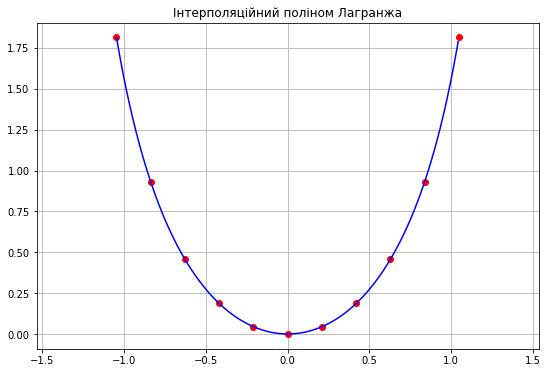
\includegraphics[width=1\linewidth]{Lagrange.png}}
    \caption{Результати інтерполяції поліномом Лагранжа}
    \label{fig:Lagrange}
\end{figure}

\newpage
\subsubsection*{Сплайн-інтерполяція}

\lstinputlisting{Code/Spline.py}

\begin{figure}[H]
    \center{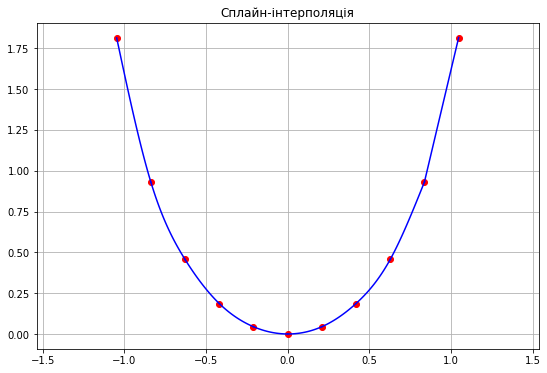
\includegraphics[width=1\linewidth]{Spline.png}}
    \caption{Результати сплайн-інтерполяції}
    \label{fig:Spline}
\end{figure}

\subsubsection*{Похибки інтеполяції}

\lstinputlisting{Code/Error.py}

\begin{figure}[H]
    \center{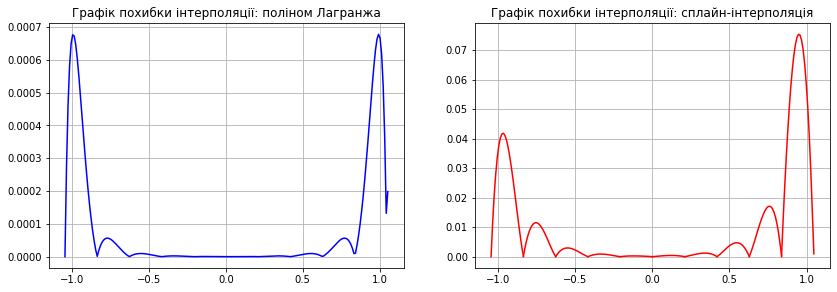
\includegraphics[width=1\linewidth]{Errors.png}}
    \caption{Графіки похибок інтерполяції}
    \label{fig:Errors}
\end{figure}

\begin{table}[H]
    \begin{center}
        \begin{tabular}{||c|c|c||}
            \hline
            \textnumero & \textbf{Спосіб інтерполяції} & \textbf{Значення похибки}\\
            \hline \hline
            $\varepsilon_1$ & Поліном Лагранжа & 0.0006779999272341 \\
            \hline
            $\varepsilon_2$ & Сплайн-інтерполяція & 0.0753149362380392 \\
            \hline
        \end{tabular}
        \caption{Значення похибок інтерполяції}
        \label{tab:errors}
    \end{center}
\end{table}

\subsection*{Контрольні запитання}

\begin{enumerate}
    \item \textit{Чи будуть відрізнятись поліноми Ньютона та Лагранжа одного степеня, побудовані для однієї 
    системи вузлів?}

    Згідно теореми про єдиність інтерполяційного поліному, поліноми Ньютона та Лагранжа одного степеня, 
    побудовані для однієї системи вузлів, відрізнятись не будуть.

    \item \textit{У чому перевага побудови поліному Ньютона порівняно із побудовою поліному Лагранжа?}
    
    У випадку побудови поліному Лагранжа додавання до системи іще одного вузла інтерполяції змусить заново 
    перераховувати й видозмінювати кожен з формуючих доданків поліному, а відтак -- і весь існуючий поліном. 
    
    Натомість в аналогічній ситуації у випадку побудови поліному Ньютона достатньо просто додати до вже 
    існуючого поліному лише один новий доданок.
    
    \item \textit{Яка кількість вузлів необхідна для побудови інтерполяційного поліному порядку $n$?}
    
    Для побудови інтерполяційного поліному порядку $n$ необхідно визначити $n+1$ вузлів інтерполяції. 
    
    \item \textit{Запишіть систему рівнянь для знаходження коефіцієнтів сплайнів другого порядку на двох 
    сусідніх відрізках.}

    Як уже зазначалося, ідея сплайн-інтерполяції полягає у побудові поліномів між парами сусідніх вузлів 
    інтерполяції, причому для кожної пари вузлів будується свій поліном. 

    Найпоширеніший у практиці є кубічний сплайн, який і був розглянутий у цьому практикумі. Стосовно ж 
    квадратичного сплайна, то для його побудови необхідно побудувати $n$ многочленів другої степені 
    такого виду:
    \[ S(x)=a_i+b_i(x-x_{i})+c_i(x-x_i)^2,\ \text{де } x_i\leqslant x\leqslant x_{i+1}\]

    Або ще зустрічається така аналогічна форма запису:
    \[ S(x)=a_i+b_i x+c_i x^2 \]

    В обидвох формах запису першочерговою задачею побудови сплайну є знаходження коефіцієнтів $a_i,b_i,c_i$. Як 
    і раніше, пошук цих величин відбувається із накладених обмежень на вираз $S(x)$:
    \begin{itemize}
        \item у сусідніх вузлах інтерполяції $x_i$ та $x_{i+1}$ побудований поліном $S(x)$ має задовільняти 
        значенням $y_i$ та $y_{i+1}$;
        \item має виконуватися умова неперервності першої похідної у вузлах інтерполяції, тобто умова 
        гладкості кривої в усіх точках. Інакше кажучи, зліва і справа від вузла інтерполяції перша похідна 
        сусідніх сплайнів має бути рівною: $S_i'(x_i)=S_{i+1}'(x_i)$.
        \item перші похідні сплайну $S(x)$ та початкової функції $F(x)$ в початковій точці $x_0$ мають збігатися: 
        $S'(x_0)=F'(x_0)$.
    \end{itemize}

    Отже, із заданих трьох умов складається система обмежень на шукані коефіцієнти $a_i,b_i,c_i$. Приклад 
    побудови квадратичного спланй розглянутий у
    \href{https://studfile.net/preview/1865619/page:2/}{цьому джерелі}. 


\end{enumerate}

\end{document}